\documentclass[11pt,a4paper]{article}

% $ProjectHeader: use 0.393 Wed, 16 May 2007 14:10:28 +0200 opti $

% $Format: "\\newcommand{\\version}{$ProjectVersion$}"$
\newcommand{\version}{0.393}

\usepackage{url,alltt}
\usepackage{amsmath}
\usepackage{makeidx}
\usepackage{graphicx}
\usepackage{graphicx}
\usepackage{times} 
%\usepackage{showidx}

% --- set margins
%\usepackage{geometry}
%\geometry{nohead,width=24cm,height=17cm}
%\usepackage{anysize}
%\marginsize{3cm}{3cm}{2cm}{2cm}

\newcommand{\Index}[1]{#1\index{#1}}
\newcommand{\keyword}[1]{{\texttt{#1}}}
\newcommand{\code}[1]{{\texttt{#1}}}
\newcommand{\trl}{{TROLL \itshape{light}}}
\newcommand{\USE}{USE}
\newcommand{\cpp}{\mbox{C$^{++}$}}
\newcommand{\davinci}{\emph{daVinci}}
\newcommand{\prompt}{\$}
\newcommand{\param}[1]{{\textit{#1}}}
\newcommand{\lbag}{\{\!\!\{}
\newcommand{\rbag}{\}\!\!\}}

% program output, examples, etc.
\newenvironment{poutput}%
{\begin{quote}\begin{footnotesize}\begin{alltt}}%
{\end{alltt}\end{footnotesize}\end{quote}}

\sloppy
\makeindex

\parindent0em
\thispagestyle{empty}
\begin{document}

%% ================================================
%\title{\USE{} -- User Manual}
%% ================================================

\vspace*{\stretch{1}}
\rule{\linewidth}{1mm}
\begin{flushright}

\includegraphics[scale=0.6]{use1}\\
\Huge \textsc{User Manual}
\end{flushright}
\rule{\linewidth}{1mm}
\vspace*{\stretch{4}}


Mark Richters \\
University of Bremen, Germany \\
Database Systems Group \\
\url{http://www.db.informatik.uni-bremen.de}\\
\url{mr@informatik.uni-bremen.de}\\


\newpage
\tableofcontents

% --------------------------------------------------

\newpage

\parindent0em
\parskip1.5ex plus0.5ex minus0.5ex

% --------------------------------------------------
\section{Introduction}
% --------------------------------------------------

(to be written)

% --------------------------------------------------
\section{A Quick Tour}
% --------------------------------------------------

The purpose of this section is to provide a brief introduction to the
central concepts of \USE{}. A small real world example is used to
illustrate how specifications can be validated with \USE{}. For the
example case study, we have chosen the domain of car rentals. We do
not, however, give a precise requirements specification since this is
out of the scope of our interest here. We assume that an analysis of
the requirements has resulted in a first model which is shown as a UML
class diagram in Fig.~\ref{fig:CarRental}. In the diagram, attributes
and operations of classes are omitted for reasons of readability.

\begin{figure}[htbp]
  \begin{center}
    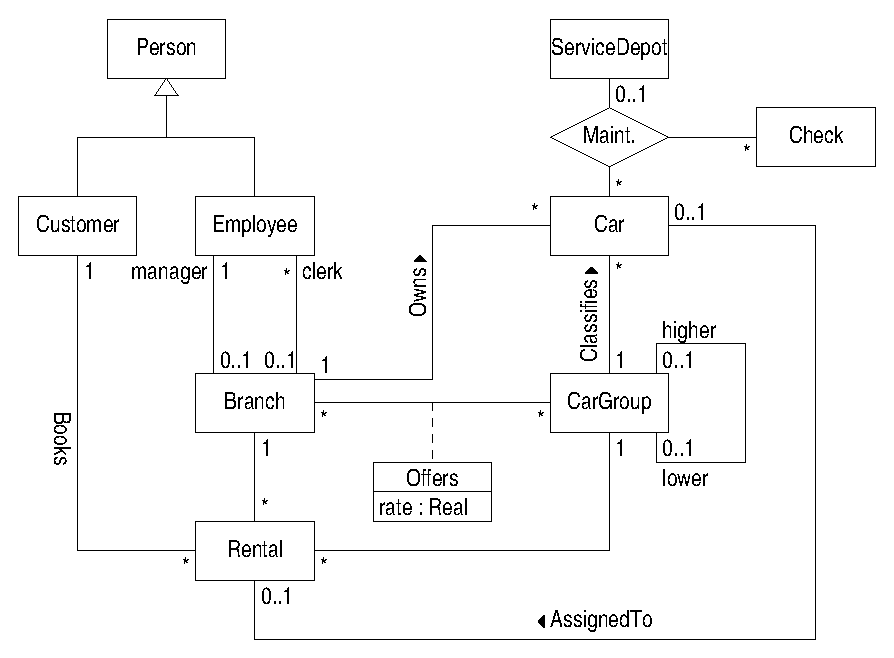
\includegraphics[width=\textwidth]{carrental2-uml}
    \caption{A Car Rental}
    \label{fig:CarRental}
  \end{center}
\end{figure}

In \USE{} you have to write a textual specification which serves as a
description of a model. The specification for the model in
Fig.~\ref{fig:CarRental} can be found in the \texttt{examples}
directory in file \texttt{CarRental2.use}. A part of the specification
describing the class Person is shown in Fig.~\ref{fig:classPerson}.

\begin{figure}[htbp]
\begin{small}
\begin{alltt}
\textbf{abstract} \textbf{class} Person
\textbf{attributes}
  firstname : String;
  lastname : String;
  age : Integer;
\textbf{operations}
  \emph{// produce a full name, e.g. 'Mr. Frank Black'}
  fullname(prefix : String) : String =
    prefix.concat(' ').concat(firstname).concat(' ').concat(lastname);
\textbf{constraints}
  \emph{// both names must be defined}
  firstname.isDefined \textbf{and} lastname.isDefined;
  \emph{// the age must be in a reasonable range}
  age > 0 \textbf{and} age < 150;
end
\end{alltt}
\end{small}
    \caption{Specification of Class Person}
    \label{fig:classPerson}
\end{figure}

The Person class is defined as being abstract, i.e.\ there may be only
instances of one of the subclasses Customer or Employee. The
attributes of a person object are its firstname, lastname and age. An
operation fullname can be used to produce e.g. an opening address in a
letter. The operations meaning is given by an OCL expression which
concatenates the argument \emph{prefix} with the attribute values of
firstname and lastname. The constraints section of the specification
contains invariants that must hold in every system state for each
object of class Person (or its subclasses). An invariant is an OCL
expression with a boolean result type.

Generally, a specification contains classes and associations to
describe the structural properties of a model. Further restrictions on
the model can be specified with OCL constraints. A specification may
contain any number of classes, associations, and constraints. 

Once you have written a specification \USE{} can help you validating
the specification by letting you instantiate the specified model.
Objects of classes can be created, and they can be linked to each
other according to the specification of associations in the model.
Objects have a state that may change over time, or objects may vanish
completely. We will see how this can be done in some more detail very
soon.

\USE{} allows you to execute a design before it is built as a software
system. This way mistakes in the specification can be corrected very
early in the software construction process. Furthermore a
specification can be tested with data expected in the final
application domain. \USE{} checks all constraints specified in your
model and informs you about states which do violate any constraint.
The result of such a constraint violation is that you will either have
to rethink your constraints (are they really adequate?) or the data
(is the data correct for your application?).

\subsection{Checking a Specification}

(to be continued)

% --------------------------------------------------

\clearpage
\addcontentsline{toc}{section}{References}
\bibliographystyle{alpha}
\bibliography{mr,abt}

\clearpage
\addcontentsline{toc}{section}{Index}
\printindex

\end{document}
